\section{Motivating Examples}

Filter reconstruction
\begin{figure}
\centering
\begin{subfigure}{.32\linewidth}
  \centering
  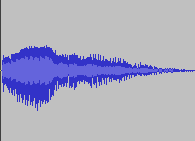
\includegraphics[width=.9\textwidth]{figs/original.png}
  \caption{Input example}
  \label{fig:inEx}
\end{subfigure}%
\begin{subfigure}{.32\linewidth}
  \centering
  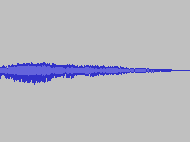
\includegraphics[width=.9\textwidth]{figs/lpf800.png}
  \caption{Output example}
  \label{fig:outEx}
\end{subfigure}
\begin{subfigure}{.32\linewidth}
  \centering
  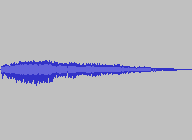
\includegraphics[width=.9\textwidth]{figs/lpf950.png}
  \caption{Generated}
  \label{fig:synthEx}
\end{subfigure}
\caption{The waveforms (a) and (b) are provided as examples, and DSP-PBE synthesizes a filter that produces (c).}
\label{fig:test}
\end{figure}

More creative applications?
